\section{Evaluation}
\subsection{Web UI showcase}
\subsection{Comparison with the official Emulator based on compatability}
\begin{itemize}
  \item Sys.wait not the same (but also different behaviour on official emulator, based on stdlib)
  \item keyboard bug for bug compatible
\end{itemize}

\subsection{Comparison with the official Emulator based on UI}
\subsubsection{Hosting the application on GitHub Pages}
\subsection{Comparison with the official Emulator based on Performance}
\subsubsection{Benchmarks} \label{sec:benchmarks}

There are two distinct modes in which the Emulators can operate: the interactive mode, in which the display memory is actually rendered to a visible canvas, and the test mode, in which a test scripts runs without any further user input to verify the correctness of a hack program.
From a performance point of view, however, only the former is relevant, since all test scripts used in the course finish so quickly that measuring the performance differences between different emulators would basically be meaningless.
So, to really evaluate the new emulators, a sufficiently complex graphical program is required. For this task, one of Gavin Stewart's impressive graphical demonstrations for the Hack platform was chosen.
The GASchunky program~\cite{demos} renders a complex animation in an infinite loop to the internal display. It requires no user input, but uses almost all of the available functionality of the platform, making it a perfect choice for benchmarking. In order to turn it into a proper benchmark, the loop was removed, leaving only a single iteration of the animation to be played.
\cref{fig:gaschunky-screenshot} shows a frame of the generated animation.
Furthermore, some modifications were made to the emulators. For both the official and new graphical emualtors, two statements have been added to the code. Both print the current system time in milliseconds and get executed when the start button is pressed and when the program returns from the main function respectively. Additionally in the third column of the ~\cref{table:gaschunky}, the one millisecond wait instruction in the FastforwardTask of the HackController.java was removed to ensure that the official emulator could run at its maximum speed.
The new emulator was run both from the web UI and in desktop mode. In both cases the tickrate was set to one million, which is ten times as much as the normal maximum tickrate in the web UI. This limit is however arbitrarily chosen and therefore does not reflect the true performance of the system. At a tick rate of one million, the viewer can still see the animation clearly, which allows for a fair comparison.

\begin{table}[ht]
  \begin{center}
    \begin{tabular}{@{}lllll@{}}
      \toprule
      Run & Official & Official (no wait) & Native &   Web \\ \midrule
      1   &   43.77s &             36.76s &  1.33s & 1.59s \\
      2   &   43.34s &             36.98s &  1.34s & 1.64s \\
      3   &   45.10s &             36.88s &  1.39s & 1.64s \\
      4   &   44.36s &             37.02s &  1.35s & 1.59s \\
      5   &   43.27s &             37.82s &  1.35s & 1.62s \\
      6   &   45.05s &             36.65s &  1.36s & 1.74s \\
      7   &   43.60s &             37.63s &  1.35s & 1.69s \\
      8   &   44.20s &             36.09s &  1.35s & 1.76s \\
      9   &   44.22s &             37.13s &  1.35s & 1.73s \\
      10  &   44.01s &             37.71s &  1.32s & 1.70s \\ \bottomrule
    \end{tabular}
    \caption{GASchunky benchmark (lower is better)}%
    \label{table:gaschunky}
  \end{center}
\end{table}

\begin{figure}[ht]
  \centering
  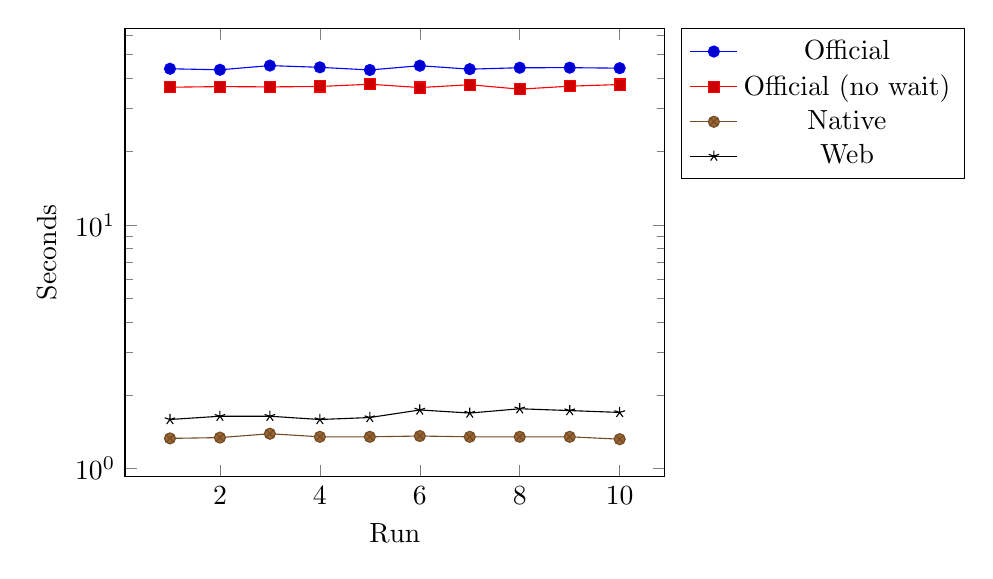
\begin{tikzpicture}
    \begin{axis}[
      ymode=log,
      ylabel=Seconds,
      xlabel=Run,
      legend pos=outer north east,
      ]
      \addplot coordinates {
        (1,  43.77)
        (2,  43.34)
        (3,  45.10)
        (4,  44.36)
        (5,  43.27)
        (6,  45.05)
        (7,  43.60)
        (8,  44.20)
        (9,  44.22)
        (10, 44.01)
      };
      \addplot coordinates {
        (1,  36.76)
        (2,  36.98)
        (3,  36.88)
        (4,  37.02)
        (5,  37.82)
        (6,  36.65)
        (7,  37.63)
        (8,  36.09)
        (9,  37.13)
        (10, 37.71)
      };
      \addplot coordinates {
        (1,  1.33)
        (2,  1.34)
        (3,  1.39)
        (4,  1.35)
        (5,  1.35)
        (6,  1.36)
        (7,  1.35)
        (8,  1.35)
        (9,  1.35)
        (10, 1.32)
      };
      \addplot coordinates {
        (1,  1.59)
        (2,  1.64)
        (3,  1.64)
        (4,  1.59)
        (5,  1.62)
        (6,  1.74)
        (7,  1.69)
        (8,  1.76)
        (9,  1.73)
        (10, 1.70)
      };
      \addlegendentry{Official}
      \addlegendentry{Official (no wait)}
      \addlegendentry{Native}
      \addlegendentry{Web}
    \end{axis}
  \end{tikzpicture}
  \caption{GASchunky benchmark (lower is better)}%
  \label{fig:gachunky-plot}
\end{figure}

It is clearly visible that the new Emulator is several times faster than the official implementation.
On average, the official emulator without modifications takes around 44 seconds to render the full animation once. Meanwhile the Web version of the new emulator manages to achieve the same result in just 1.7 seconds on average. The native version of the new emulator which uses SDL to render the internal display is even faster, just taking 1.35 seconds on average. While the official emulator can be sped up drastically, it still does not come close.
This shows us that even though the new emulator only uses a single thread and runs in a browser, it still offers massive performance benefits over the official implementation.
